\chapter{溶解离子型固体和分子型固体}\label{ch:g11:dissolution}

一小撮食盐搅入水中，几秒钟便消失不见；同样一小撮
食盐搅入食用油中，却原封不动地沉在杯底，
无论观察多久都是如此。油腻的锅在水龙头下冲洗，依旧油腻；
滴入一滴洗洁精，油污便脱离了锅面。什么因素决定
一种物质能否\omterm{def:g2:mixing-and-dissolving:dissolve}{溶解}于液体中？答案
在于上一章中的\omterm{def:g11:polarity-and-cohesion:polar-bond}{部分电荷}
和粒子之间的作用力。

\begin{recall}
\omterm{def:g6:solutions-and-solubility:solubility}{溶解度}；\omterm{def:g6:solutions-and-solubility:miscible}{互溶的}液体与\omterm{def:g6:solutions-and-solubility:miscible}{不互溶的}液体
（见\cref{ch:g6:solutions-and-solubility}）。\omterm{def:g9:ions:ionic-compound}{离子化合物}由
\omterm{def:g9:ions:ion}{阳离子}和\omterm{def:g9:ions:ion}{阴离子}按比例构成，使其呈电中性
（见\cref{ch:g9:ions}）。\omterm{def:g11:polarity-and-cohesion:polar-molecule}{极性分子}与\omterm{def:g11:polarity-and-cohesion:polar-molecule}{非极性分子}、\omterm{def:g11:polarity-and-cohesion:hydrogen-bond}{氢键}、
范德华相互作用（见\cref{ch:g11:polarity-and-cohesion}）。
\omterm{def:g10:chemical-species:extraction}{液–液萃取}（见\cref{ch:g10:chemical-species}）。
\omterm{def:g10:concentration-and-dilution:molar-concentration}{物质的量浓度}（见\cref{ch:g10:concentration-and-dilution}）。
\end{recall}

\section{溶解离子型固体}

在氯化钠晶体中，每个钠\omterm{def:g9:ions:ion}{离子} \ce{Na+} 周围都有
氯\omterm{def:g9:ions:ion}{离子} \ce{Cl-}，每个氯\omterm{def:g9:ions:ion}{离子}周围都有钠\omterm{def:g9:ions:ion}{离子}，它们依靠
异种电荷之间的吸引力结合在一起。极性的水\omterm{def:g7:atoms-and-molecules:molecule}{分子}
受到这些电荷的吸引：其氧端（$\delta^-$）指向\omterm{def:g9:ions:ion}{阳离子}，
氢端（$\delta^+$）指向\omterm{def:g9:ions:ion}{阴离子}。

\begin{definition}[解离]\label{def:g11:dissolution:dissociation}
\omterm{def:g9:ions:ion}{离子}型固体在\omterm{def:g6:solutions-and-solubility:solute}{溶剂}中的\emph{解离}\index{解离}，是指
其中的\omterm{def:g9:ions:ion}{离子}彼此分开：它们离开晶体，
在溶液中相互远离。
\end{definition}

\begin{definition}[溶剂化、水合]\label{def:g11:dissolution:solvation}
\omterm{def:g2:mixing-and-dissolving:dissolve}{溶解}后的粒子被\omterm{def:g6:solutions-and-solubility:solute}{溶剂}\omterm{def:g7:atoms-and-molecules:molecule}{分子}包围，二者靠吸引作用结合，这一过程
称为\emph{溶剂化}\index{溶剂化}；在水中则称为\emph{水合}\index{水合}。
化学式后面的符号 (aq) 表示
“水合”。
\end{definition}

\begin{proposition}[溶解的三个阶段]\label{prop:g11:dissolution:stages}
\omterm{def:g9:ions:ion}{离子}型固体溶于水时，同时经历三个阶段：\omterm{def:g9:ions:ion}{离子}从晶体中被拉出
（\omterm{def:g11:dissolution:dissociation}{解离}）、被水\omterm{def:g7:atoms-and-molecules:molecule}{分子}包围（\omterm{def:g11:dissolution:solvation}{水合}），并扩散到整个溶液中（分散）。
以氯化钠为例，
其\omterm{def:g2:mixing-and-dissolving:dissolve}{溶解}过程可表示为
\[
  \ce{NaCl(s) -> Na+(aq) + Cl-(aq)} .
\]
\end{proposition}

\begin{proof}
在本阶段不加证明地承认：\omterm{def:g9:ions:ion}{离子}与极性水\omterm{def:g7:atoms-and-molecules:molecule}{分子}之间的吸引作用，
加起来足以取代
晶体中\omterm{def:g9:ions:ion}{离子}之间的作用。
\end{proof}

\begin{omfigure}
\begin{tikzpicture}[font=\small]
  % the crystal edge: alternating ions
  \foreach \i in {0,1,2,3,4} \foreach \j in {0,1,2,3} {
    \pgfmathtruncatemacro\k{mod(\i+\j,2)}
    \ifnum\k=0
      \node[om atom, ball color=green!60!black, minimum size=6.4mm] at (0.8*\i,0.8*\j) {};
    \else
      \node[om atom, ball color=violet!70, minimum size=4.0mm] at (0.8*\i,0.8*\j) {};
    \fi
  }
  % a hydrated Na+ that has left: O towards the ion
  \begin{scope}[shift={(5.6,1.8)}]
    \node[om atom, ball color=violet!70, minimum size=4.0mm] (na) at (0,0) {};
    \node[font=\footnotesize] at (0,0) {};
    \foreach \a in {0,90,180,270} {
      \node[aO, minimum size=4.6mm] (o\a) at (\a:0.62) {};
      \node[aH, minimum size=3.2mm] (ha\a) at ($(\a:0.62)+(\a+52:0.42)$) {};
      \node[aH, minimum size=3.2mm] (hb\a) at ($(\a:0.62)+(\a-52:0.42)$) {};
      \begin{scope}[on background layer]
        \draw[bond, line width=1.2pt] (o\a.center) -- (ha\a.center);
        \draw[bond, line width=1.2pt] (o\a.center) -- (hb\a.center);
      \end{scope}
    }
    \node[anchor=north] at (0,-1.35) {\ce{Na+(aq)}};
  \end{scope}
  % a hydrated Cl- that has left: H towards the ion
  \begin{scope}[shift={(8.6,1.4)}]
    \node[om atom, ball color=green!60!black, minimum size=6.4mm] at (0,0) {};
    \foreach \a in {45,135,225,315} {
      \node[aH, minimum size=3.2mm] (h\a) at (\a:0.62) {};
      \node[aO, minimum size=4.6mm] (o\a) at (\a:1.0) {};
      \node[aH, minimum size=3.2mm] (k\a) at ($(\a:1.0)+(\a+75:0.42)$) {};
      \begin{scope}[on background layer]
        \draw[bond, line width=1.2pt] (o\a.center) -- (h\a.center);
        \draw[bond, line width=1.2pt] (o\a.center) -- (k\a.center);
      \end{scope}
    }
    \node[anchor=north] at (0,-1.45) {\ce{Cl-(aq)}};
  \end{scope}
  \node[anchor=north, align=center] at (1.6,-0.45) {晶体 \\
    （\ce{Na+} 较小，\ce{Cl-} 较大）};
\end{tikzpicture}

{\small 氯化钠的\omterm{def:g2:mixing-and-dissolving:dissolve}{溶解}。一个钠\omterm{def:g9:ions:ion}{离子}和一个氯\omterm{def:g9:ions:ion}{离子}已离开晶体，
各自已被\omterm{def:g11:dissolution:solvation}{水合}。在\omterm{def:g9:ions:ion}{阳离子}周围，水\omterm{def:g7:atoms-and-molecules:molecule}{分子}将氧\omterm{def:g7:atoms-and-molecules:atom}{原子}（红色，$\delta^-$）
朝内排列；在\omterm{def:g9:ions:ion}{阴离子}周围，水\omterm{def:g7:atoms-and-molecules:molecule}{分子}将氢\omterm{def:g7:atoms-and-molecules:atom}{原子}（白色，$\delta^+$）
朝内排列。}
\end{omfigure}

\section{离子的浓度}

\begin{method}[每种离子的浓度]\label{met:g11:dissolution:ions}
\begin{enumerate}
  \item 写出配平的\omterm{def:g2:mixing-and-dissolving:dissolve}{溶解}方程式（\omterm{def:g7:atoms-and-molecules:atom}{原子}数与电荷数均守恒）：
        对于氯化钙，\ce{CaCl2(s) -> Ca^{2+}(aq) + 2Cl-(aq)}。
  \item 计算\omterm{def:g2:mixing-and-dissolving:dissolve}{溶解}的固体的\omterm{def:g10:the-mole:amount}{物质的量} $n$，
        则溶液中\omterm{def:g6:solutions-and-solubility:solute}{溶质}的浓度为 $c = n / V$。
  \item 每种\omterm{def:g9:ions:ion}{离子}的浓度等于 $c$ 乘以其在方程式中的\omterm{def:g8:balanced-equations:coefficient}{化学计量数}：
        此处 $[\ce{Ca^{2+}}] = c$，
        $[\ce{Cl-}] = 2c$。
\end{enumerate}
方括号 $[\ldots]$ 表示
某种\omterm{def:g2:mixing-and-dissolving:dissolve}{溶解}的\omterm{def:g6:pure-substances-and-mixtures:species}{化学物种}的\omterm{def:g10:concentration-and-dilution:molar-concentration}{物质的量浓度}。
\end{method}

\begin{example}[氯化钙]\label{ex:g11:dissolution:cacl2}
% ledger: aw:Ca, aw:Cl
\qty{5.55}{g} 氯化钙（$M = \qty{111.1}{g/mol}$）\omterm{def:g2:mixing-and-dissolving:dissolve}{溶解}
配成 \qty{500.0}{mL} 溶液：$n = \qty{0.0500}{mol}$，
$c = \qty{0.100}{mol/L}$，故 $[\ce{Ca^{2+}}] = \qty{0.100}{mol/L}$，
$[\ce{Cl-}] = \qty{0.200}{mol/L}$。溶液呈电中性：每升中正电荷为 $2 \times
0.100$，负电荷为 $1 \times 0.200$。
\end{example}

\section{极性与溶解度}

\begin{proposition}[相似相溶]\label{prop:g11:dissolution:like}
极性\omterm{def:g6:solutions-and-solubility:solute}{溶剂}（如水）能\omterm{def:g2:mixing-and-dissolving:dissolve}{溶解}\omterm{def:g9:ions:ion}{离子}型固体和极性
物质，尤其是能与之形成\omterm{def:g11:polarity-and-cohesion:hydrogen-bond}{氢键}的物质；非极性\omterm{def:g6:solutions-and-solubility:solute}{溶剂}
（如环己烷或植物油）能\omterm{def:g2:mixing-and-dissolving:dissolve}{溶解}非极性物质。
\omterm{def:g9:ions:ion}{离子}型固体在非极性\omterm{def:g6:solutions-and-solubility:solute}{溶剂}中\omterm{def:g2:mixing-and-dissolving:dissolve}{溶解}很少，
非极性物质在水中也\omterm{def:g2:mixing-and-dissolving:dissolve}{溶解}很少。
\end{proposition}

\begin{proof}
在本阶段不加证明地承认：\omterm{def:g6:solutions-and-solubility:solute}{溶质}与\omterm{def:g6:solutions-and-solubility:solute}{溶剂}之间能形成的吸引作用，
至少不弱于\omterm{def:g6:solutions-and-solubility:solute}{溶质}自身粒子之间以及\omterm{def:g6:solutions-and-solubility:solute}{溶剂}\omterm{def:g7:atoms-and-molecules:molecule}{分子}之间被拆散的作用时，
\omterm{def:g6:solutions-and-solubility:solute}{溶质}便能良好地\omterm{def:g2:mixing-and-dissolving:dissolve}{溶解}。
\end{proof}

\begin{example}[三种情形]\label{ex:g11:dissolution:cases}
% ledger: sol:I2-water, sol:I2-heptane
乙醇与水以任意比例互溶：其 \ce{O-H} 基团与水形成
\omterm{def:g11:polarity-and-cohesion:hydrogen-bond}{氢键}。盐溶于水，但不溶于油。
碘，\ce{I2}，为\omterm{def:g11:polarity-and-cohesion:polar-molecule}{非极性分子}，在水中\omterm{def:g6:solutions-and-solubility:solubility}{溶解度}很小（约
\qty{0.3}{g/L}，溶液呈棕色），但在非极性\omterm{def:g6:solutions-and-solubility:solute}{溶剂}中\omterm{def:g6:solutions-and-solubility:solubility}{溶解度}较大
（每千克庚烷中可溶 \qty{17}{g}，溶液呈紫色）。
\end{example}

\section{液–液萃取详解}

\omterm{def:g10:chemical-species:extraction}{液–液萃取}是将某物质从一种\omterm{def:g6:solutions-and-solubility:solute}{溶剂}转移到
另一种与前者不互溶、且该物质在其中\omterm{def:g6:solutions-and-solubility:solubility}{溶解度}更大的\omterm{def:g6:solutions-and-solubility:solute}{溶剂}中。
“相似相溶”的规则可用来判断应选择哪种\omterm{def:g6:solutions-and-solubility:solute}{溶剂}。

\begin{inthelab}[萃取碘]
将 \qty{20}{mL} 棕色的碘\omterm{def:g6:solutions-and-solubility:solute}{水溶液}与
\qty{10}{mL} 环己烷一同倒入分液漏斗，塞紧塞子，
振荡，经活塞放气，然后
静置，分为两层：密度较小的环己烷在上层。上层
现呈紫色，下层几乎无色：碘已转入
环己烷中。下层经活塞放出，
碘便保留于环己烷中。
\end{inthelab}

\begin{omfigure}
\begin{tikzpicture}[font=\small, scale=1.15]
  \pic[transform shape] at (0,0) {sepfunnel={orange!55!brown!70}{white}};
  \node[anchor=north, align=center] at (0,-0.15) {振荡前};
  \draw[omProp, <-] (0.55,2.1) -- (1.4,2.5) node[right, text=black] {环己烷};
  \draw[omProp, <-] (0.45,1.35) -- (1.4,1.2) node[right, text=black,
    align=left] {棕色碘水};
  \pic[transform shape] at (4.6,0) {sepfunnel={orange!10}{violet!60}};
  \node[anchor=north, align=center] at (4.6,-0.15) {振荡并 \\ 静置后};
  \draw[omProp, <-] (5.15,2.1) -- (6.0,2.5) node[right, text=black,
    align=left] {环己烷中的碘 \\ （紫色）};
  \draw[omProp, <-] (5.05,1.35) -- (6.0,1.2) node[right, text=black,
    align=left] {水，几乎 \\ 无色};
\end{tikzpicture}

{\small 用环己烷从水中萃取碘。非极性的碘
转入非极性\omterm{def:g6:solutions-and-solubility:solute}{溶剂}中；环己烷密度小于水，
漂浮在上层。}
\end{omfigure}

\begin{safety}{\ghs[0.82cm]{GHS02}\ghs[0.82cm]{GHS07}\ghs[0.82cm]{GHS08}\ghs[0.82cm]{GHS09}}
% ledger: ghs:I2, ghs:cyclohexane
环己烷极易燃，其蒸气使人昏昏欲睡，吞食后对肺部有害，
且对水生生物毒性很大。碘
经皮肤接触或吸入有害。操作时使用通风橱、护目镜和
手套，附近严禁明火；有机废液须收集。
\end{safety}


\section{肥皂与两亲分子}

\begin{definition}[亲水性与疏水性]\label{def:g11:dissolution:hydrophilic}
某物质或\omterm{def:g7:atoms-and-molecules:molecule}{分子}的一部分若能被水吸引，则称其为\emph{亲水的}\index{亲水的}
（如\omterm{def:g9:ions:ion}{离子}基团、极性基团，或能形成\omterm{def:g11:polarity-and-cohesion:hydrogen-bond}{氢键}的基团）；
若不能被水吸引，则称其为\emph{疏水的}\index{疏水的}
（由碳\omterm{def:g7:atoms-and-molecules:atom}{原子}和氢\omterm{def:g7:atoms-and-molecules:atom}{原子}构成的长链，非极性）。疏水物质
易溶于油脂。
\end{definition}

\begin{definition}[两亲分子与胶束]\label{def:g11:dissolution:amphiphilic}
\emph{两亲的}\index{两亲的}\omterm{def:g7:atoms-and-molecules:molecule}{分子}或\omterm{def:g9:ions:ion}{离子}具有一个
亲水头部与疏水尾部。在水中，两亲\omterm{def:g9:ions:ion}{离子}会聚集成
\emph{胶束}\index{胶束}：微小的球体，尾部在内，
远离水，
头部位于表面，与水接触。
\end{definition}

\begin{example}[一种肥皂]\label{ex:g11:dissolution:soap}
% ledger: aw:C, aw:H, aw:O, aw:Na
硬脂酸钠，\ce{C17H35COONa}（$M = \qty{306.0}{g/mol}$），是一种
典型肥皂，由动植物油脂制得。在水中，它\omterm{def:g2:mixing-and-dissolving:dissolve}{溶解}为
钠\omterm{def:g9:ions:ion}{离子} \ce{Na+} 和硬脂酸根\omterm{def:g9:ions:ion}{离子} \ce{C17H35COO-}：其头部为
\ce{-COO-}，具有\omterm{def:g9:ions:ion}{离子}性、亲水性；尾部为 17 个碳\omterm{def:g7:atoms-and-molecules:atom}{原子}，
\omterm{def:g11:dissolution:hydrophilic}{疏水的}。
\end{example}

\begin{omfigure}
\begin{tikzpicture}[font=\small]
  % the stearate ion as a zigzag of 17 carbons + COO-
  \foreach \k in {0,1,2,3,4,5,6,7,8,9,10,11,12,13,14,15,16} {
    \pgfmathsetmacro\y{mod(\k,2)==0 ? 0 : 0.3}
    \coordinate (c\k) at (0.42*\k,\y);
  }
  \draw[line width=0.9pt] (c0) \foreach \k in {1,2,3,4,5,6,7,8,9,10,11,12,13,14,15,16} { -- (c\k) };
  \coordinate (cc) at ($(c16)+(30:0.42)$);
  \begin{scope}[on background layer]
    \fill[omDef!15, rounded corners] ($(cc)+(-0.25,-0.55)$) rectangle ($(cc)+(1.05,0.9)$);
  \end{scope}
  \draw[line width=0.9pt] (c16) -- (cc);
  \draw[line width=0.9pt] (cc) -- ++(90:0.4) node[above] {O};
  \draw[line width=0.9pt] ([xshift=1.5pt]cc) -- ++(90:0.36);
  \draw[line width=0.9pt] (cc) -- ++(-30:0.42) node[right] {O$^-$};
  \draw[omProp] ($(c0)+(0,-0.15)$) -- ++(0,-0.15) -- ($(c16)+(0,-0.3)$) -- ++(0,0.15);
  \node[omProp, anchor=north] at ($(c8)+(0,-0.32)$) {疏水尾部（17 个碳原子）};
  \node[omDef, anchor=south] at ($(cc)+(0.35,0.9)$) {亲水头部};
  % the sketch
  \begin{scope}[yshift=-1.9cm]
    \draw[omProp, line width=1.6pt, decorate, decoration={snake, amplitude=1.5pt,
      segment length=6pt}] (2.0,0) -- (5.2,0);
    \fill[omDef] (5.45,0) circle (0.25);
    \node[white, font=\scriptsize\bfseries] at (5.45,0) {$-$};
    \node[anchor=west] at (5.9,0) {同一离子的示意};
  \end{scope}
\end{tikzpicture}

{\small 硬脂酸根\omterm{def:g9:ions:ion}{离子}。在这个锯齿形画法中，链上每个拐角都是一个碳\omterm{def:g7:atoms-and-molecules:atom}{原子}，
带有氢\omterm{def:g7:atoms-and-molecules:atom}{原子}（\ce{CH2}，链远端为 \ce{CH3}）。后面的章节会解释这种简写。
下面是常见的示意图：
一条波浪形的尾部和一个圆形的头部。}
\end{omfigure}

\begin{proposition}[肥皂如何去除油污]\label{prop:g11:dissolution:soap}
油脂是\omterm{def:g11:dissolution:hydrophilic}{疏水的}，不溶于水。在肥皂水中，
肥皂\omterm{def:g9:ions:ion}{离子}的尾部\omterm{def:g2:mixing-and-dissolving:dissolve}{溶解}在油脂中，而头部
留在水中；油脂被分散成细小的液滴，每个液滴都被一个
\omterm{def:g11:dissolution:amphiphilic}{胶束}包裹，其带电表面朝向水，这些液滴
随冲洗的水被带走。
\end{proposition}

\begin{proof}
在本阶段不加证明地承认：这由“相似相溶”应用于\omterm{def:g9:ions:ion}{离子}的两端得出；
外侧的带电头部还能阻止液滴
重新合并，因为同种电荷相互排斥。
\end{proof}

\begin{omfigure}
\begin{tikzpicture}[font=\small]
  \fill[yellow!45!orange!35] (0,0) circle (1.0);
  \node at (0,0) {油脂};
  \foreach \a in {0,20,40,60,80,100,120,140,160,180,200,220,240,260,280,300,320,340} {
    \draw[omProp, line width=1.3pt, decorate, decoration={snake,
      amplitude=1pt, segment length=4pt}] (\a:0.55) -- (\a:1.45);
    \fill[omDef] (\a:1.6) circle (0.15);
  }
  \node[anchor=west, align=left] at (2.4,0.6) {头部（$-$）在水中};
  \node[anchor=west, align=left] at (2.4,-0.4) {尾部在油脂中};
  \draw[black!50] (2.4,0.6) -- (1.75,0.45);
  \draw[black!50] (2.4,-0.4) -- (1.05,-0.25);
  \node[font=\small, blue!50!black] at (-2.6,1.4) {水};
\end{tikzpicture}

{\small \omterm{def:g11:dissolution:amphiphilic}{胶束}截面图：肥皂\omterm{def:g9:ions:ion}{离子}包围着一个油脂液滴，
尾部朝内，带电的头部朝外。每个\omterm{def:g11:dissolution:amphiphilic}{胶束}表面都带负电，
\omterm{def:g11:dissolution:amphiphilic}{胶束}之间相互排斥。}
\end{omfigure}

\begin{omfigure}
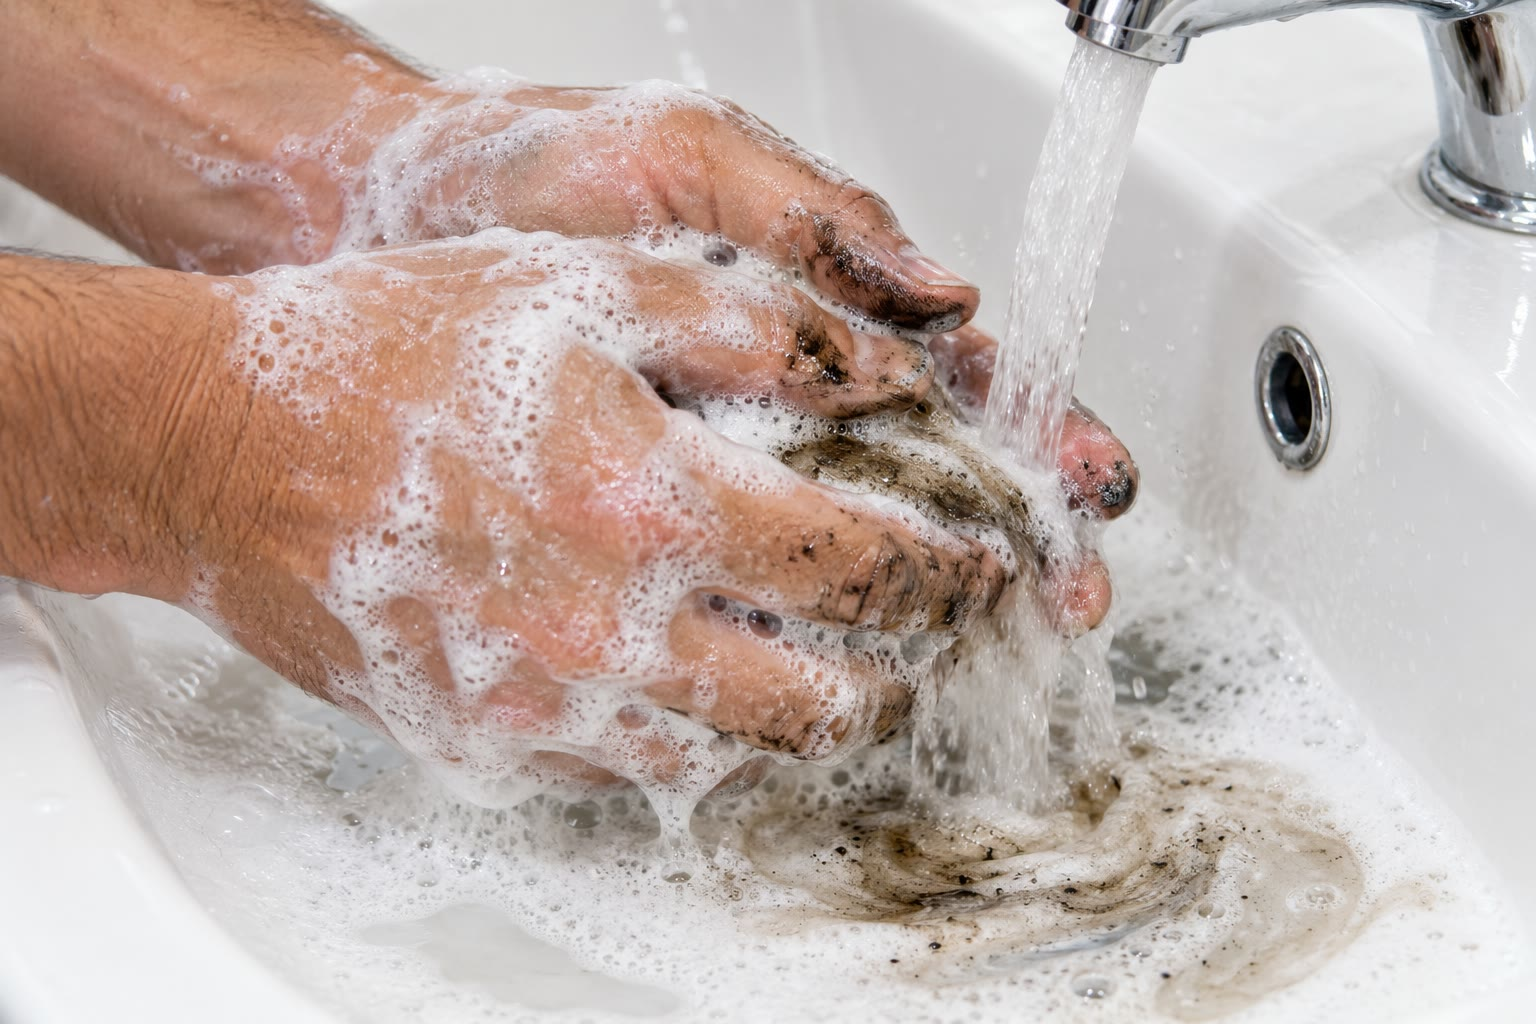
\includegraphics[width=0.48\linewidth]{images/book1/ai/g11-greasy-hands.jpg}

{\small 洗涤沾有油污的手：肥皂通过\omterm{def:g11:dissolution:amphiphilic}{胶束}将油脂带走。}
\end{omfigure}

\begin{remark}[硬水与浮渣]\label{rem:g11:dissolution:scum}
硬水中含有大量钙\omterm{def:g9:ions:ion}{离子} \ce{Ca^{2+}} 和镁\omterm{def:g9:ions:ion}{离子}
\ce{Mg^{2+}}，它们从水流经的岩石中溶出。与硬脂酸根\omterm{def:g9:ions:ion}{离子}
结合生成\omterm{def:g9:ions:precipitate}{沉淀}（见\cref{ch:g9:ions}），即硬脂酸钙：
\[
  \ce{2C17H35COO- + Ca^{2+} -> Ca(C17H35COO)2(s)} .
\]
这种灰白色固体就是洗脸盆边缘的浮渣，每一个
被它捕获的肥皂\omterm{def:g9:ions:ion}{离子}都无法再用于去污：在硬水中，肥皂起泡很差，
直到加入足量的肥皂使全部钙\omterm{def:g9:ions:ion}{离子}\omterm{def:g9:ions:precipitate}{沉淀}为止。
\end{remark}

\begin{omfigure}
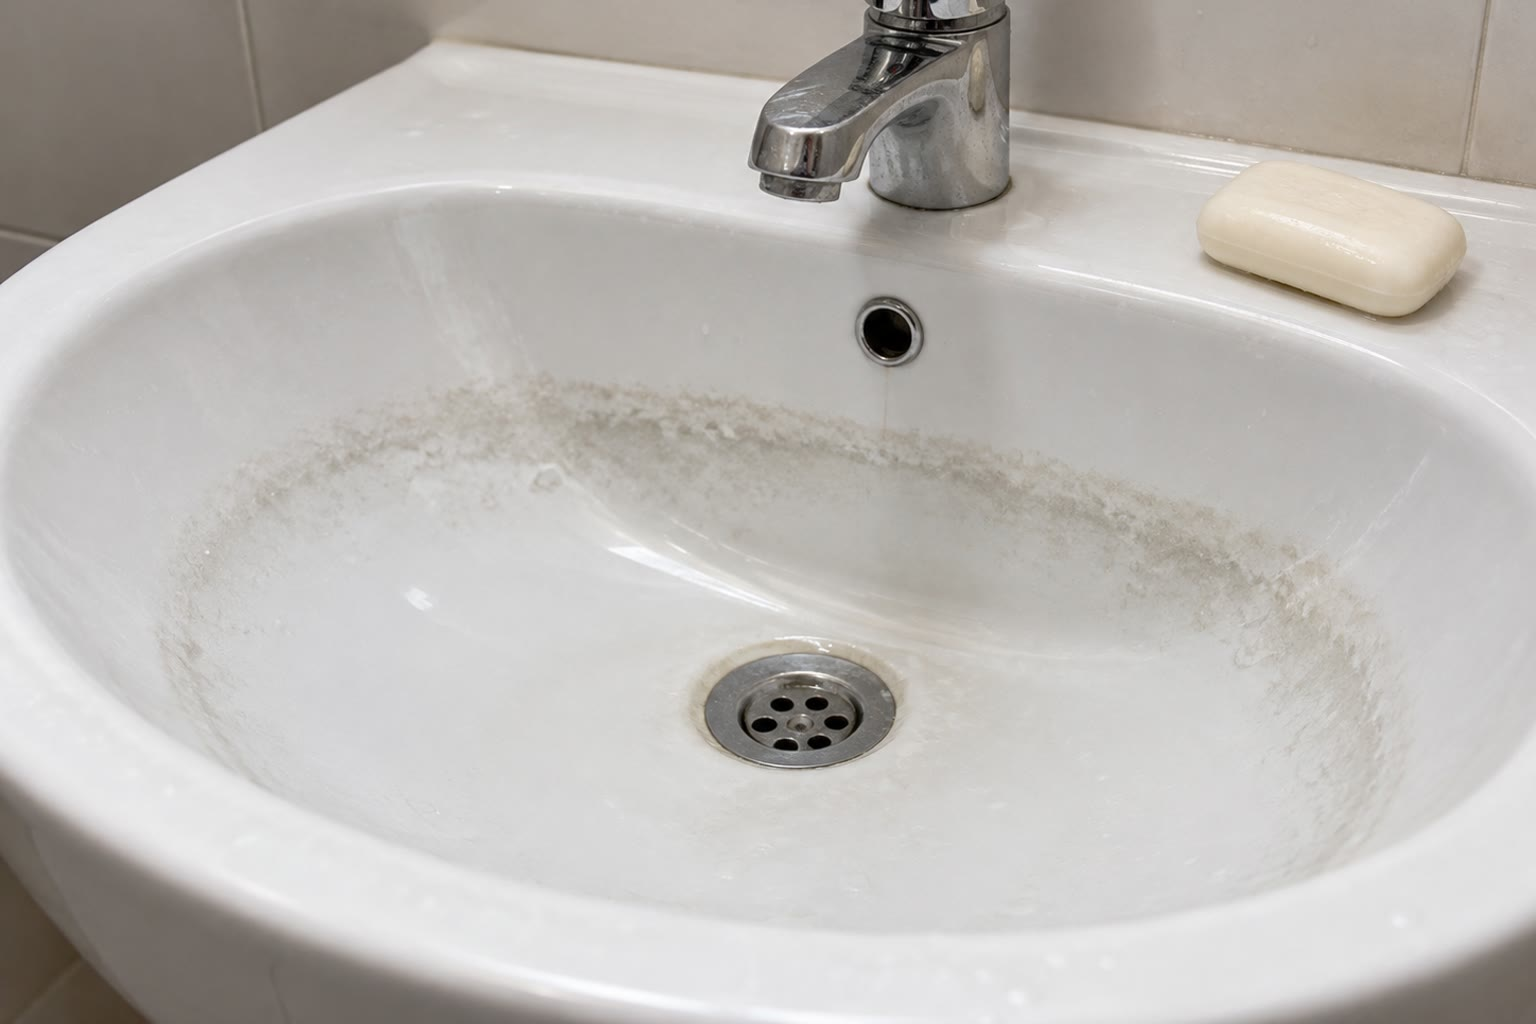
\includegraphics[width=0.45\linewidth]{images/book1/ai/g11-soap-scum.jpg}

{\small 洗脸盆中的浮渣：硬脂酸钙，是由硬水
中的钙\omterm{def:g9:ions:ion}{离子}\omterm{def:g9:ions:precipitate}{沉淀}而成。}
\end{omfigure}

\section{练习}


\begin{exercise}[$\star$]\label{exo:g11:dissolution:1}
写出下列物质在水中\omterm{def:g2:mixing-and-dissolving:dissolve}{溶解}的方程式：氯化钠 \ce{NaCl}、
氯化钙 \ce{CaCl2}、硫酸钠 \ce{Na2SO4} 和氯化铝
\ce{AlCl3}。
\end{exercise}

\begin{exercise}[$\star$]\label{exo:g11:dissolution:2}
硫酸钠溶液中 $c = \qty{0.050}{mol/L}$，
求钠\omterm{def:g9:ions:ion}{离子}和硫酸根\omterm{def:g9:ions:ion}{离子}的浓度。
\end{exercise}

\begin{exercise}[$\star$]\label{exo:g11:dissolution:3}
什么是\omterm{def:g9:ions:ion}{离子}的\omterm{def:g11:dissolution:solvation}{水合}？水\omterm{def:g7:atoms-and-molecules:molecule}{分子}的哪一端指向\omterm{def:g9:ions:ion}{阳离子}，
哪一端指向\omterm{def:g9:ions:ion}{阴离子}？为什么？
\end{exercise}

\begin{exercise}[$\star$]\label{exo:g11:dissolution:4}
将 \qty{2.67}{g} 氯化铝\omterm{def:g2:mixing-and-dissolving:dissolve}{溶解}，配成
\qty{200.0}{mL} 溶液，求该溶液的浓度
及每种\omterm{def:g9:ions:ion}{离子}的浓度。
\end{exercise}

\begin{exercise}[$\star$]\label{exo:g11:dissolution:5}
指出硬脂酸根\omterm{def:g9:ions:ion}{离子}各部分是\omterm{def:g11:dissolution:hydrophilic}{亲水的}还是\omterm{def:g11:dissolution:hydrophilic}{疏水的}，
并说明理由。
\end{exercise}

\begin{exercise}[$\star\star$]\label{exo:g11:dissolution:6}
应选用水还是环己烷作\omterm{def:g6:solutions-and-solubility:solute}{溶剂}来\omterm{def:g2:mixing-and-dissolving:dissolve}{溶解}：食盐；
蜡烛中的石蜡（长链烃）；蔗糖（含有许多 \ce{O-H} 基团）；
碘？逐一说明你的选择理由。
\end{exercise}

\begin{exercise}[$\star\star$]\label{exo:g11:dissolution:7}
乙醇 \ce{CH3-CH2-OH} 能与水以任意比例互溶，而己烷
\ce{C6H14} 与水不互溶。试解释原因。
\end{exercise}

\begin{exercise}[$\star\star$]\label{exo:g11:dissolution:8}
观察\omterm{def:g11:dissolution:amphiphilic}{胶束}的截面图。为什么尾部在内侧，头部
在外侧？为什么两个\omterm{def:g11:dissolution:amphiphilic}{胶束}不会合并成一个更大的油滴？
\end{exercise}

\begin{exercise}[$\star\star$]\label{exo:g11:dissolution:9}
某植物的香气成分溶于水中。要将其萃取出来，化学家可以用
乙醇或环己烷。哪一种合适，另一种为何不合适
（考虑互溶性）？
\end{exercise}

\begin{exercise}[$\star\star$]\label{exo:g11:dissolution:10}
在碘的萃取实验中，环己烷层为何位于上层？哪一层
从分液漏斗的活塞放出？最后碘存在于何处？
\end{exercise}

\begin{exercise}[$\star\star$]\label{exo:g11:dissolution:11}
将硫酸铜的蓝色溶液与环己烷一起振荡。
其蓝色会发生什么变化？请解释。
\end{exercise}

\begin{exercise}[$\star\star\star$]\label{exo:g11:dissolution:12}
欲配制 \qty{250.0}{mL} 溶液，需\omterm{def:g2:mixing-and-dissolving:dissolve}{溶解}氯化钙的质量为多少，
使溶液中 $[\ce{Cl-}] = \qty{0.300}{mol/L}$？
\end{exercise}

\begin{exercise}[$\star\star\star$]\label{exo:g11:dissolution:13}
经测定，某海水样品中含 \qty{0.010}{mol/L} 的钙\omterm{def:g9:ions:ion}{离子}
和 \qty{0.053}{mol/L} 的镁\omterm{def:g9:ions:ion}{离子}。请解释普通肥皂为何在海水中起泡很差，
并求出仅由一升海水中的钙\omterm{def:g9:ions:ion}{离子}
所能\omterm{def:g9:ions:precipitate}{沉淀}的硬脂酸钠的量为多少？
\end{exercise}

\begin{exercise}[$\star\star\star$]\label{exo:g11:dissolution:14}
\qty{100.0}{mL} 的氯化钠溶液，浓度为
\qty{0.20}{mol/L}，与 \qty{100.0}{mL} 的氯化钙溶液\omterm{def:g2:mixing-and-dissolving:mix}{混合}，
其浓度为 \qty{0.10}{mol/L}。未生成\omterm{def:g9:ions:precipitate}{沉淀}。求\omterm{def:g2:mixing-and-dissolving:mix}{混合}液中
\ce{Na+}、\ce{Ca^{2+}} 和 \ce{Cl-} 的浓度，并检验溶液是否
呈电中性。
\end{exercise}

\begin{exercise}[$\star\star\star$]\label{exo:g11:dissolution:15}
% ledger: sol:I2-water, sol:I2-heptane, rho:heptane
碘在水中的\omterm{def:g2:mixing-and-dissolving:dissolve}{溶解}量约为每升 \qty{0.3}{g}，在庚烷中约为每千克
\qty{17}{g}。已知庚烷的密度约为
\qty{0.68}{kg/L}。一升庚烷能\omterm{def:g2:mixing-and-dissolving:dissolve}{溶解}的碘量
是一升水的多少倍？这对萃取意味着什么？
\end{exercise}

\section{问题：肥皂与硬水}

\begin{problem}[{周末问题——一浴缸硬水会因生成
浮渣而浪费多少肥皂？}]
\label{pb:g11:dissolution:1}
% ledger: aw:Ca, aw:Mg, aw:C, aw:H, aw:O, aw:Na
某自来水每升含 \qty{120}{mg} 钙\omterm{def:g9:ions:ion}{离子}和 \qty{24}{mg}
镁\omterm{def:g9:ions:ion}{离子}。浴缸中注入 \qty{150}{L} 这种水，洗澡者
使用由硬脂酸钠 \ce{C17H35COONa} 制成的肥皂。

\medskip
\noindent\textbf{部分 I——水中有什么。}
\begin{enumerate}
  \item 自来水中的钙\omterm{def:g9:ions:ion}{离子}和镁\omterm{def:g9:ions:ion}{离子}从何而来？
  \item 计算钙\omterm{def:g9:ions:ion}{离子}和
        镁\omterm{def:g9:ions:ion}{离子}的\omterm{def:g10:concentration-and-dilution:molar-concentration}{物质的量浓度}。
  \item 钙\omterm{def:g9:ions:ion}{离子}伴随有碳酸氢根\omterm{def:g9:ions:ion}{离子}，
        \ce{HCO3-}，仿佛\omterm{def:g2:mixing-and-dissolving:dissolve}{溶解}了碳酸氢钙 \ce{Ca(HCO3)2}。
        写出该\omterm{def:g2:mixing-and-dissolving:dissolve}{溶解}方程式，并推出与
        钙\omterm{def:g9:ions:ion}{离子}相伴的碳酸氢根\omterm{def:g9:ions:ion}{离子}的
        浓度。
  \item 浴缸中含有钙\omterm{def:g9:ions:ion}{离子}的\omterm{def:g10:the-mole:amount}{物质的量}为多少？
\end{enumerate}

\medskip
\noindent\textbf{部分 II——肥皂。}
\begin{enumerate}[resume]
  \item 计算硬脂酸钠的\omterm{def:g10:the-mole:molar-mass}{摩尔质量}。
  \item 写出其在水中的\omterm{def:g2:mixing-and-dissolving:dissolve}{溶解}方程式。
  \item 硬脂酸根\omterm{def:g9:ions:ion}{离子}的哪一部分是\omterm{def:g11:dissolution:hydrophilic}{亲水的}，哪一部分
        是\omterm{def:g11:dissolution:hydrophilic}{疏水的}？为何称其为\omterm{def:g11:dissolution:amphiphilic}{两亲的}？
  \item 描述\omterm{def:g11:dissolution:amphiphilic}{胶束}，并解释它如何将油脂从
        皮肤上去除。
  \item 洗涤时，为何肥皂必须溶于水而非油中？
\end{enumerate}

\medskip
\noindent\textbf{部分 III——浮渣。}
\begin{enumerate}[resume]
  \item 写出硬脂酸钙\omterm{def:g9:ions:precipitate}{沉淀反应}的方程式。
        检验方程式两边电荷是否守恒。
  \item 对 \qty{1.00}{L} 自来水及过量的硬脂酸根\omterm{def:g9:ions:ion}{离子}，填写
        \omterm{def:g10:reaction-progress-table:extent}{进度表}。哪一种\omterm{def:g7:chemical-reactions:reactant}{反应物}为\omterm{def:g10:reaction-progress-table:limiting}{限量反应物}？
  \item 每升水中，有多少\omterm{def:g10:the-mole:amount}{物质的量}的硬脂酸根\omterm{def:g9:ions:ion}{离子}因与钙\omterm{def:g9:ions:ion}{离子}结合而损失？
  \item 计算硬脂酸钙的\omterm{def:g10:the-mole:molar-mass}{摩尔质量}，以及每升生成的
        浮渣的质量。
  \item 硬脂酸镁以相同方式\omterm{def:g9:ions:precipitate}{沉淀}。镁\omterm{def:g9:ions:ion}{离子}每升
        需结合多少\omterm{def:g10:the-mole:amount}{物质的量}的硬脂酸根\omterm{def:g9:ions:ion}{离子}？
\end{enumerate}

\medskip
\noindent\textbf{部分 IV——浴缸。}
\begin{enumerate}[resume]
  \item 整个浴缸中的钙\omterm{def:g9:ions:ion}{离子}能\omterm{def:g9:ions:precipitate}{沉淀}
        多少\omterm{def:g10:the-mole:amount}{物质的量}的硬脂酸根\omterm{def:g9:ions:ion}{离子}？
  \item 这相当于多少质量的肥皂？
  \item 加上镁\omterm{def:g9:ions:ion}{离子}，共浪费多少质量的肥皂？
  \item 一块肥皂约重 \qty{100}{g}。仅钙\omterm{def:g9:ions:ion}{离子}
        就需消耗多少块肥皂？
  \item 给出最终结论：这种水装满一个
        \qty{150}{L} 的浴缸时，钙\omterm{def:g9:ions:ion}{离子}以浮渣形式浪费多少质量的肥皂？
\end{enumerate}
\end{problem}
